\chapter{Combat}
\label{ch:combat}

Fantasy D100 is a swords and sorcery game and, as such, swords will be drawn during epic quests with the aim of spilling blood. Be it for glory, honour, fame or riches, when all else fails violence is the means of achieving these goals. The characters come from worlds that are rife with conflict, where warriors are required to wage wars against evil neighbours, wandering bandits and foul monsters that come out of the wilderness.  

It should be remembered that Fantasy D100 is not a game purely about combat, just as it is not purely about magic. It would not be unusual for whole sessions to pass without any physical violence. However, in time, characters will get involved in dangerous life threatening fights. 

This chapter provides you with a straightforward and direct system for playing out action packed and deadly combat.

\section{Combat is Tough}
Characters that have weapon skills less than 100\% are at the whim of the dice to determine whether or not they land a blow in combat. Anything you do to increase your character’s chances to hit, or hit first, will stand in your favour and make the outcome more certain.

Once you are hit in combat, things start getting messy. Your character has a relatively low number of hit points. In a couple of blows, or one lucky blow, these hit points can easily be reduced to zero, which indicates that the character has died. Make sure your character can dodge, parry or has magical protection. With Major Wounds your character is especially at risk of grievous and permanent harm every time they decide to use violence to solve a problem.

Numbers count. If you are facing off against multiple opponents, even weak and unskilled ones, you are quickly going to run out of attacks and reactions. In practical terms this means that your character may, at best, reduce the number of attackers by one per round, while only being able to protect themselves against one of several incoming attacks. 

Even Masters are vulnerable. A weapon skill over 100\% is no guarantee of survival, as characters can be brought low by a lucky critical hit, or by an opponent who has lured them into an ambush and stacked the odds against them through surprise and careful planning. 

These harsh realities mean that players tend to avoid combats where they do not have a very good chance to win. Instead of wading into masses of weaker opponents, hoping that lucky dice rolls will see them through, they carefully plan ambushes, where they have the benefit of terrain and supporting soldiers from the local militia that will allow them to wipe out the majority of the enemy before the first proper round of combat. They will use any of their Powers to boost their damage, chances to hit, or armour and in general try to get an advantage.


\section{Summary of Combat}
\begin{description}
	\item[Work out encounter distance:] The Gamemaster determines how far away the hostile group is to the player characters, either at Range or Close.

	\item[Start Combat time:] Combat is divided into rounds. A single round has a duration of five seconds of time, giving 12 rounds in every minute. During a round every character can perform one action. Combat rounds cycle through the following steps:
	\begin{rpg-list}
	\item Determine Order: At the start of every combat, check each character’s DEX (or INT if they are spell casting) +1D6; this is their Combat Order and will determine the order in which every character involved acts for the round.
	\item Characters Take Action \& Reaction: In a combat round each character gets one Combat Action and one Defensive Reaction. Combat Actions, such as attacks, take place in Combat Order. The character with the highest order will act first, followed by the character with the second-highest order, and so on until the character with the lowest order acts. Reactions, such as parries or dodges, are made during this process as they are needed.
	\item End of Combat Round: Once all eligible characters have acted in the combat round, it is over. If there are characters still engaged in combat with enemies, another combat round begins. 
	\end{rpg-list}
\end{description}

\begin{rpg-examplebox}
For example: Lura has DEX 15 and rolled a 3 for a total of 18 Combat Order. A Goblin has DEX 13 and rolled a 4 for a total of 17. Thus the Combat Order is Lura acting before the Goblin.
\end{rpg-examplebox}

\section{Encounter Distance}
Not all combats start with the two sides, the players and their opponents, directly facing each other within swords reach.  At the beginning of a combat, or potential combat, the Gamemaster must determine which of the two distances the encounter starts at.

Close is a range of two metres or less and is the distance at which a character can engage in either Close or Unarmed combat. 

Ranged, beyond two metres up to double the range of the missile weapon a character is holding, is the distance at which the character can engage in ranged combat. Ranged combat typically happens out in the open countryside where groups of combatants can see each over coming over the horizon or emerging in the distance from old ruined buildings.


\subsection{Some Basic Rules}
\begin{rpg-list}
\item A Combat Round lasts five seconds.

\item You get one Combat Action, usually an attack, and one Defensive Reaction, usually a defensive action, per combat round.

\item You can move your Movement Rate in a Combat Round without losing your Action or Reaction. 

\item You can run twice your Movement Rate in a Combat Round but you may only Dodge as your Reaction.

\item To defend or attack you roll against your Close Combat, Ranged Combat or Unarmed Combat skill depending on the type of weapon you are using.

\item When attacked you can either Parry (use the Close Combat or Unarmed skill) or Dodge as a Reaction.

\item If your character successfully Dodges an attack they take no damage.

\item If your opponent successfully Parries your attack their weapon or shield reduces the damage your attack does.

\item If you successfully hit, your opponent takes damage to their hit points equal to 
	Weapon Damage rolled + your Damage Modifier - (Opponent’s Armour Points)
\end{rpg-list}

\begin{figure*}%[h]
\begin{center}
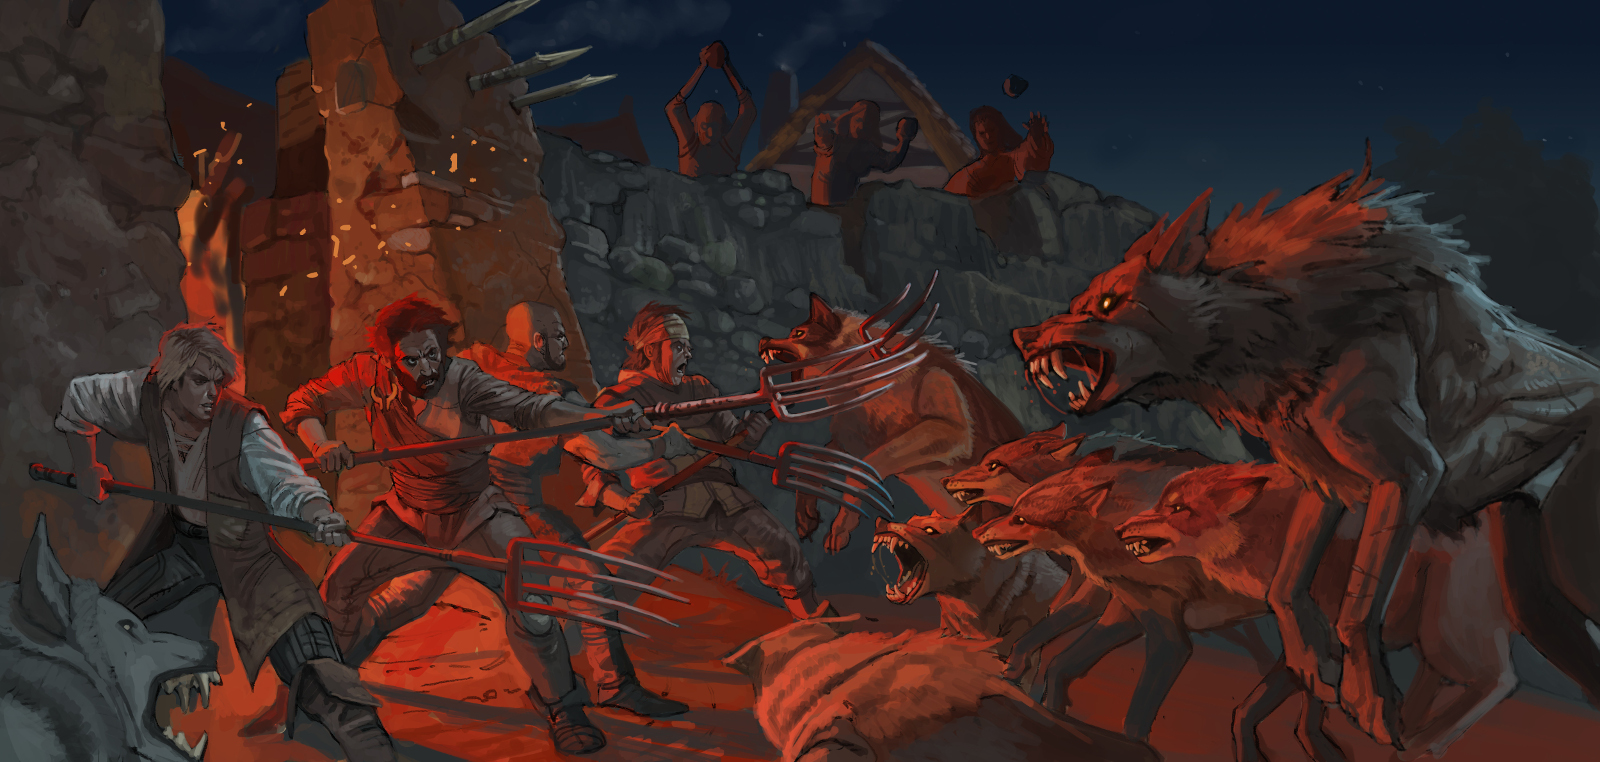
\includegraphics[scale=1.3]{img/fending_off_the_wolves_by_ncorva.jpg}
\end{center}
\end{figure*}


\section{Combat Actions}
The actions a character may take when it is his turn to act are detailed here. A character can only choose one of the options below each round.

\subsection{Close Combat Actions}
\begin{description}
	\item[Charge:]  If a character can move a minimum of five metres towards his opponent, then he can make a charge. He may move a distance up to - but no more than - twice his Movement Rate.  This must be in a straight line and he must end up adjacent to an enemy.  When the move is complete, a close combat attack may be made against the enemy. If the attack is successful, the character gains a bonus of +1D6 damage. He loses his defensive reaction for the round that he charges on. Characters may not charge uphill and gain the damage modifier.
	\item[Close Combat Attack:]  The character can make a single close combat attack. In addition to the normal attack, there are the following special attacks.
		\begin{rpg-list}
		\item All out Attack: The attacker gives up their Reaction for the round but gains a second attack, which happens straight after the first attack. Both attacks are at -20\% due to the loss of skill during this frenzied attack. This type of attack cannot be combined with Great Attack or Disarming Attack.
\item Great Attack: This attack is made using swords, axes or maces where the attacker has enough room to wind up the weapon for a really forceful blow. The attacker gains a +20\% to attack and automatically does the maximum damage modifier value but loses his reaction for that combat round.
\item Disarming Attack: Attacker attacks at -20\% to his weapon skill with the aim of disarming their opponent either of their weapon or shield. If the attack is successful and the opponent fails to parry or dodge, the weapon or shield is thrown 1D6 metres away from the owner. 
\item Knockout Attack: Attacker attacks at -20\% to his weapon skill with the aim of knocking out their opponent. If the attack is successful and the opponent fails to parry or dodge, and the damage done is equal to a major wound then the opponent is knocked out without suffering any damage. If the damage is equal to a minor wound the opponent takes the minimum damage of the weapon but is not knocked out.
\item Knock-Back Attack: Requires a successful shield attack (with a -20\% if in off-hand). If the opponent fails to parry or dodge he takes no damage but is knocked-back 2 metres. The opponent needs to make an Athletics roll at -20\% or also fall prone.
		\end{rpg-list}
	\item[Intimidate/Persuade:]  The character tries to get the other side to surrender or flee. This can either be targeted at a single enemy or a group.  Do an Opposed roll using the character’s Influence vs. the enemies’ Persistence, modified as listed below. Groups roll once using the Persistence of the group leader. If the group leader’s Influence skill is higher than his Persistence, then they may use that skill instead. Apply the following modifiers to the enemy’s skill depending on the state of the enemy.
	\begin{rpg-table}[|c|X|]
		\hline
		+40\% & if the enemy is still at full strength, or has only taken some minor wounds.\\
		+20\% & if the enemy out numbers the player’s side, but have had at least 20\% losses either in numbers or hit points.\\
		-20\% & if the enemy is fewer than the player’s side and has taken some wounds.\\
		-40\% & if the enemy has taken more than half hit points in wounds and/or has seen half his group incapacitated by the players.\\
		\hline
		\multicolumn{2}{|p{\linewidth-4.5mm}|}{Note: these modifiers are not cumulative. Apply the one that best describes the situation.}\\
		\hline
	\end{rpg-table}

If the enemy is at full strength and/or outnumbers the player characters then only a critical roll for Influence vs a failed Persistence roll will make them surrender.  A fumbled Persistence roll will see the enemy suddenly rout.

When the player is attempting the roll they must declare whether they are targeting the whole group or singling out an individual.  The Gamemaster has the final say on who is targeted and if if attempt is possible at all. 

	\begin{rpg-examplebox}
Rurik is fighting a group of four goblins, one of whom he has already badly wounded while the other three are still at full hit points. 

If he decides to single out the wounded Goblin, then the Goblin’s Persistence roll to resist Rurik’s taunting and the resultant urge to flee will be at -20\%. If he decides to target the whole group, which as a whole is undamaged and outnumbers him, then the Goblins will be at +20\% to their Persistence. 
	\end{rpg-examplebox}

The character need not speak the same language as the opponent they are trying to Influence, but they must be capable of some sort of sign, gesture or body language that the opponent is capable of understanding.

	\item[Set Weapon:]  A character can spend their Action setting the shaft of a weapon, such as a spear or polearm, in the ground in anticipation of a charge from an opponent. When the charge actually comes the character automatically gets an attack at +20\% before the charging character gets their attack. If the character makes any other action or reaction before the charge, the weapon becomes ‘unset’.
\end{description}


\subsubsection{Making Close Combat Attacks}
\begin{rpg-list}
\item Making the Attack: To attack, the player simply rolls 1D100 and compares it to the character’s Close Combat skill which may be modified for the specific situation or special attack being attempted. If a character rolls equal to or lower than his Weapon skill, he has hit his target. If a character rolls greater than his Weapon skill, he has missed his target. 

\item Target Reaction: If the enemy has already reacted this round, or chooses not to React against this attack, then this attack is unopposed. Move straight on to Damage Resolution. If the attack is opposed, the defender makes a Dodge or Parry (see below).

\item Damage Resolution: If the attack is successful, damage is rolled. Each weapon has its own Damage score, to which the attacker’s Damage Modifier is added in order to determine the total damage being dealt. If the defender is armoured then the armour will absorb some of this damage. Reduce the attack’s damage by the armour points (AP) of the defender’s armour. 

\item Damage Application: Apply any remaining damage to the defender’s hit points. 
\end{rpg-list}

\begin{table}
\begin{center}
\caption{Close Combat Situational Modifiers}
\label{tab:close-combat-situational-modifiers}
\begin{rpg-table}[|X|c|]
        \hline
        \textbf{Situation} & \textbf{Skill Modifier}\\
        \hline
        Target is helpless  & Automatic Critical\\
        Target is prone or attacked from behind & +20\%\\
	Attacking or defending while on higher ground or on mount (unless wielding a weapon two size categories smaller) & +20\%\\
        Attacking or defending while prone & -20\%\\
        Attacking or defending while on unstable ground & -20\%\\
        Attacking or defending while underwater & -40\%\\
	Defending while on lower ground or against mounted foe (unless wielding a weapon two size categories larger) & -20\%\\
        Fighting in partial darkness & -20\%\\
        Fighting in darkness & -40\%\\
        Fighting in pitch dark or blinded & -60\%\\
        \hline
\end{rpg-table}
\end{center}
\end{table}



\begin{table*}
\begin{center}
\caption{Summary of Combat Results}
\label{tab:combat-results}
\begin{rpg-table}[|l|l|X|]
        \hline
        \textbf{Attacker} & \textbf{Defender's Reaction} & \textbf{Result}\\
        \hline
        Fumble   & No need to roll & Attacker funbles.\\
        Failure  & No need to roll & Attacker fails to hit defender.\\
        Success  & Fumble          & Attacker hits, defender takes damage rolled minus armour points and fumbles.\\
        Success  & Failure         & Attacker hits, defender takes damage rolled minus armour points.\\
        Success  & Success         & If dodging defender avoids the attack. If parrying then if attacker’s weapon smaller or equal in size to defender’s weapon all damage avoided. If parrying weapon is a rank smaller half damage, if two ranks smaller then no damage can be avoided.\\
        Success  & Critical        & Defender avoids attack and takes no damage. If parrying the weapon size penalty does not come into it.\\
        Critical & Fumble          & Attacker does maximum damage and ignores defender’s armour. Defender fumbles.\\
        Critical & Failure         & Attacker does maximum damage and ignores defender’s armour.\\
        Critical & Success         & Similar to Success:Failure above.\\
%        Critical & Success         & Attacker does maximum damage minus defender’s armour points.\\
        Critical & Critical        & Similar to Success:Success above.\\
        \hline
\end{rpg-table}
\end{center}
\end{table*}


\subsection{Unarmed Combat Actions}
The following are potential actions:
\begin{description}
\item[Unarmed Combat Attack:] The character can make a single Unarmed Combat Attack.
\item[Natural Weapon attack:] Using the characters’s natural weapons be it claw, bite, kick or fist.
\item[Grapple Attack:] The attacker attempts to grab an opponent and an opposed Unarmed Combat Attack is made. If the attacker wins they may choose to inflict pain, immobilise or throw their opponent.
\end{description}

\subsubsection{Making Unarmed Combat Attacks}
Roll against Unarmed Combat skill to determine if the attack is successful. If an Unarmed Attack is parried by a crafted or natural weapon, then the attacker will immediately suffer the rolled damage of the parrying weapon, with no damage modifier. This is in addition to the normal effect of the parry. 

\subsubsection{Natural Weapons}
Natural Weapons such as the teeth and claws of monsters are counted as weapons and not Unarmed Attacks. The damage they deal is listed in the monster’s description. They may parry other Natural Weapons or Unarmed Attacks, but not crafted weapon attacks.

\subsubsection{Damage Modifier}
Damage Modifier is applied normally to Unarmed Combat.

\subsubsection{Grappling}
Grapple Attack is made in the same way as a normal Unarmed or Natural Weapon attack but must be declared as such before any dice are rolled. Should the attacker hit with his grapple attack, no damage is initially caused. Instead, the attacker then opposes his Unarmed Combat Skill to the target’s Unarmed Combat Skill, in a roll similar to an opposed skill test:
\begin{rpg-list}
\item \textbf{Grapple Fails:} The grapple attempt fails and the attack is considered to have missed. 
\item \textbf{Grapple Succeeds:} The two combatants are now grappling and the attacker may immediately follow up on this success by Throwing, Inflicting pain, Disarm or Immobilise the target.
\end{rpg-list}


\begin{description}
\item[Break Free:] To break out of a grapple, the character makes an opposed Grapple Attack. The characters may only use the Unarmed Combat Skill in this case. If the character succeeds they managed to break free and the combatants are no longer grappling, though they will be adjacent.
\item[Immobilise:] While immobilised, enemies are considered helpless. Once per round the defender may attempt to break free.
\item[Inflict Pain:] The grappler inflicts damage of 1D4 + damage modifiers.  Armour does not help. Once per round the defender may attempt to break free or may attempt to turn the tables on their attacker by counter grappling.
\item[Throw:] The opponent is thrown 2 metres and suffers 1D4 damage. Armour does not help. The grapple ends in this case.
\item[Disarm:] The opponent is forced to drop whatever was holding.
\end{description}

The difference in SIZ between characters matters considerably. %The Gamemaster discression is important here but as a general guideline the larger character gets a +20\% to their grapple check for every 7 points of SIZ difference they have from their opponent.
Consult table~\ref{tab:grappling-modifiers} for some guidelines. For greater differences the Gamemaster will determine if it makes sense to roll dice.

\begin{table}
\begin{center}
\caption{Grappling Modifiers}
\label{tab:grappling-modifiers}
	\begin{rpg-table}[|X|c|]
	\hline
        \textbf{Situation} & \textbf{Skill Modifier}\\
	\hline
        Attacker is $1/3$ larger in SIZ   & +20\%\\
        Attacker is $1/2$ larger in SIZ   & +40\%\\
        %Defender is $1/3$ smaller in SIZ  & -20\%\\
        %Defender is $1/2$ smaller in SIZ  & -40\%\\
	\hline
\end{rpg-table}
\end{center}
\end{table}



\subsection{Ranged Combat Actions}

The following are potential actions:
\begin{description}
\item[Ranged Combat Attack:] The character can make a single ranged combat attack. In addition to the normal attack, there is also the following special attack.
\item[Aim:] If a character aims for a round he adds a +20\% bonus to the character’s Ranged Combat skill. This bonus only applies to the first attack the character makes with the weapon, which must be fired at the target being aimed at. A character can take no Reaction while aiming without losing the aim bonus.
\end{description}

\subsubsection{Throwing Close Combat Weapons}
If a close combat weapon that isn’t designed to be thrown is hurled at an enemy then it has a range of 8m and suffers a penalty to the attack equal to its ENC x 10. Ranged Combat skill is used. 

\subsubsection{Using Ranged Weapons}
All ranged attacks are handled in same manner as close combat attacks, with the following exceptions: 
\begin{description}
\item[Charge:] Ranged attacks may not be used as part of a charge.
\item[Range:] A target within the weapon’s range may be attacked without penalty. A target within double the weapon’s range may be attacked, but the attacker’s weapon skill is halved before other modifiers are applied. Attacks cannot be made at a distance beyond twice/double the weapon’s range.
\item[Dodging and Parrying:] The target may attempt to Parry or Dodge a hand thrown ranged attack at -20\% but may not normally Dodge or Parry ranged missile weapons (such as Bows and Crossbow fire). Shield-carrying characters may Parry hand thrown missile weapons with no penalty.
\item[Disarming:] A character may not attempt to disarm targets with ranged attacks, nor may he attempt to strike a target’s weapon or shield.
\item[Damage Modifier:] A character may not add their Damage modifier to Ranged weapons except if they are Thrown weapons.

\end{description}

\subsubsection{Cover}
Cover affects both ranged and close combat attacks. For missile attacks the defender benefits from the best of the shield modifier (see section~\ref{sec:defensive-reactions}) and the cover modifier below.

\begin{description}
	\item[Partial cover (-20\%):] For example a low wall that protects the legs leaving only head and torso exposed.
	\item[Very good cover (-40\%):] For example a defender on a castle wall, firing from protected battlements.
	\item[Virtual total cover (-80\%):] For example a castle wall with arrow slits for defenders to shot through.
\end{description}


\begin{table}[H]
\begin{center}
\caption{Ranged Attack Situational Modifiers}
\label{tab:ranged-attack-situational-modifiers}
	\begin{rpg-table}[|p{5cm}|Y|]
	\hline
        \textbf{Situation} & \textbf{Skill Modifier}\\
	\hline
	\multicolumn{2}{|p{\linewidth-4.5mm}|}{Wind$^{1}$}\\
	\hline
        High wind    & -20\%\\
        Fierce wind  & -60\%\\
        Hurricane    & Attack automatically fails\\
	\hline
	\multicolumn{2}{|p{\linewidth-4.5mm}|}{Target Movement$^{1}$}\\
	\hline
        Target has moved 10m or more since attacker's last Combat Action  & -20\%\\
        Target has moved 30m or more since attacker's last Combat Action  & -40\%\\
	\hline
	\multicolumn{2}{|p{\linewidth-4.5mm}|}{Target Visibility$^{1}$}\\
	\hline
        Target obscured by smoke, mist or is in partial darkness          & -20\%\\
        Target obscured by thick smoke, fog or is in darkness             & -40\%\\
        Target is above SIZ 20                                            & +20\%\\
	\hline
	\multicolumn{2}{|p{\linewidth-4.5mm}|}{Target Condition$^{1}$}\\
	\hline
        Target is helpless                                                & +40\%\\
        Target is prone                                                   & -20\%\\
	\hline
	\multicolumn{2}{|p{\linewidth-4.5mm}|}{Attacker Condition$^{2}$}\\
	\hline
        Attacker is prone                                                 & -40\%\\
	Attacker is underwater$^{3}$                                      & -20\%\\
	Attacker is on unstable ground                                    & -20\%\\
	Attacker is blinded$^{4}$                                               & -80\%\\
	\hline
	\multicolumn{2}{|p{\linewidth-4.5mm}|}{1. Modifiers within these sections are not cumulative. However, modifiers from different sections are cumulative. Therefore, shooting at a target within a mist that has moved more than 10m since the attacker’s last Combat Action imparts a –40\% penalty.}\\
	\multicolumn{2}{|p{\linewidth-4.5mm}|}{2. Attacker condition modifiers are cumulative.}\\
	\multicolumn{2}{|p{\linewidth-4.5mm}|}{3. Only bows and crossbows may be used underwater.}\\
	\multicolumn{2}{|p{\linewidth-4.5mm}|}{4.~GMs discretion depending on the distance and the ranged weapon.}\\
	\cline{1-2}
\end{rpg-table}
\end{center}
\end{table}

\begin{figure}[H]
\begin{center}
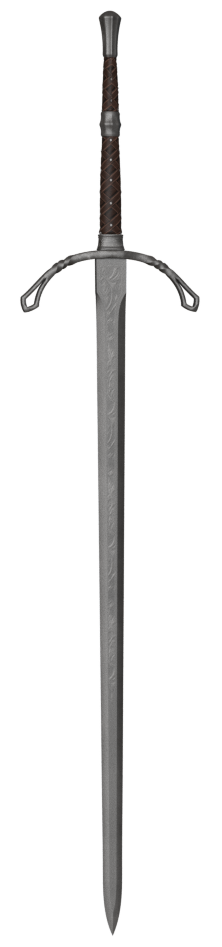
\includegraphics[scale=0.16]{img/LongSword.png}
\end{center}
\end{figure}



\subsubsection{Firing into a Crowd}
When firing into a crowd, the Gamemaster will determine how much cover the target has from the ranged attack. The ranged attack is then resolved as normal for a target behind cover. 

If the attack fails to hit the target and succeeds against the unmodified attack skill, the firer has hit one of the individuals adjacent to the target chosen by the Gamemaster. 
%The accidental target may dodge against this attack as normal. 


\subsection{Movement Actions}
A character may make one of the following Move Actions and unless noted otherwise does not lose either their Action or Reaction:

\begin{description}
\item[Change Stance:] A character may stand up from prone, or vice versa.
\item[Fighting Retreat:] A character may move a distance up to their full Movement directly away from an enemy he is fighting. He may only defend at +20\% (+40\% with a Medium and Large shield).
\item[Standard Move:] A character may move a distance up to his Movement Rate.
\item[Sprint:] A character may move a distance up to twice their Movement Rate, forsaking their attack and only being able to dodge as a defensive reaction.
\item[Ready Weapon:] Drawing a sword from its sheath, unhooking an axe from one’s belt, nocking an arrow to one’s bow – all these actions take half of available movement. A single Ready Weapon action can also include dropping a weapon currently held to the floor and then drawing a new one. Sheathing one weapon and drawing another requires the full movement as does readying two weapons. 
\end{description}


\subsection{Other Actions}

\begin{description}
\item[Powers:] This depends on which Discipline the Power belongs to. Consult the appropriate Discipline chapter.
\item[Delay:] A character may pause to assess the tactical situation around him. If a delaying character merely wishes to act after a specific character has acted, they wait until that character has finished their Combat Action. If a delaying character wishes to interrupt a specific character’s action as it occurs, the character must make a test appropriate to his interrupting action (a weapon skill test if the character wishes to attack, for instance). Whoever wins the test acts first. 
\item[Load Crossbow:] A light crossbow requires a full combat round to load while a heavy requires two full combat rounds.
\item[Skill Use:] The character performs one action which requires the use of a skill, such as opening a locked door with the Mechanisms skill.
\end{description}


\section{Defensive Reactions}
\label{sec:defensive-reactions}
A character can make one Reaction in a combat round. Unlike Combat Actions, Reactions are made in response to the successful hits of enemies. There are two types of Reaction, dodge and parry:

\begin{description}
	\item[Parries] can be made against close combat attacks. A character can also parry hand thrown missile weapons at a -20\% or without penalty if using a shield. Shields with a size of Large or Huge (i.e. Medium and Large Shields) provide a cover modifier to the ranged attack of the attacker of -20\% and -40\% respectively against arrows, sling shot and crossbow bolts. 
	\item[Dodges] can be made normally against close combat attacks and at a -20\% penalty for thrown missile weapons providing the target is aware of the attack.  
\end{description}

\noindent Reactions are declared after a successful attack has occurred but before its effects are applied. Resolution depends on the level of success between the participants and is described in table~\ref{tab:combat-results}.

%\subsection{Parry}
%When an attacker successfully hits, the defender may choose to Parry with a weapon or shield as his reaction to avoid damage. The defender rolls against their Close Combat skill. 

%If the defender succeeds then, depending on the relative weapons used, they may be able to reduce or remove all from the rolled damage. Weapons are rated in the following size categories: Light, Medium, Heavy and Huge. Weapons need to be of the same category or larger to block all damage. If the defending weapon is one category less they block half damage. If two categories less they cannot block the damage.

%A critical parry against a normal success deflects all the damage regardless of size category. If, parrying against a critical hit, the defender rolls a critical on their Close Combat skill roll then they avoid damage depending on weapon size difference.


%\subsection{Dodge}
%When an attacker successfully hits, the defender may choose to Dodge as his reaction, in order to avoid damage. The defender rolls against his Dodge skill.

%If the defender succeeds then they have successfully avoided the attack. 

%If dodging against a Critical Hit, then if the defender rolls a critical on their dodge they avoid damage. If the defender fails his dodge against a Critical Hit, the attacker does maximum damage and ignores defender’s armour.

%\subsection{Parry or Dodge?}
%What’s the difference between Parry and Dodge? Mainly down to a matter of combat style and Parrying has the advantage that it is based off the same skill that is used to Attack with, so for the purposes of skill advancement it is easier  to advance Close Combat or Unarmed than Dodge with a separate Combat skill. But remember that Dodge can be used to avoid falling rocks, traps, etc., so should not be neglected too much.


\section{Critical Hits}
Every attack skill a character possesses has a critical score. A critical score is the attack skill’s score, divided by ten, and rounded to the nearest whole number. It represents a lucky and effective hit in an unprotected area of an opponent.

If the D100 attack roll is not only lower than the attack skill, but also equal to or lower than the character’s critical score with that skill, then the attack is considered a critical hit. 

A critical hit automatically causes maximum damage for the weapon and maximum Damage Modifiers. If the character has a negative damage modifier (i.e. -1D4 or –1D6) it is not rolled for a critical hit. Critical hits also ignore armour.

\begin{rpg-examplebox}
 Rurik with his 55\% Close Combat, rolls a 05, which is a critical! He is wielding a Longsword with a damage of 1D8 and has a damage modifier of 1D6. He is fighting a heavily armoured Knight, who has the latest Plate Mail armour (AP 6). However this Armour is completely ignored as Rurik’s sword slides through a gap in the plates doing a devastating 14 points of damage (8 from the sword and 6 from the damage modifier).
\end{rpg-examplebox}

A critical hit is avoided only by a critical parry (weapon categories apply) or dodge.



\section{Fumbles}
Conversely if an attacker or defender fumbles by rolling 00, the character has been put at a severe disadvantage. It is up to the Gamemaster to determine how, dependant on the situation. Here are some examples:
\begin{rpg-list}
	\item Grievously hurt self or nearby friend with weapon, roll damage and ignore armour.
	\item Trip over and fall prone, missing one combat round.
	\item Armour or shield strap breaks, lose armour protection.
\end{rpg-list}



\section{Damage}
When a character successfully scores damage against a target it must be deducted from the target’s hit points. Every weapon has a damage rating, which is listed in its statistical entry in the relevant weapon table in the Equipment chapter. This rating is the amount of dice rolled when the weapon successfully hits a target. The attacker’s Damage Modifier is usually added to this. All damage is taken away from Hit Points. 

\begin{description}
	\item[Last hit point.] The character falls prone and will stay conscious only with a critical Resilience test roll.
	\item[Hit points equal zero.] The character is dead. However, you can spend Hero Points to avoid death.
\end{description}


\subsection{Major Wounds}
If the character takes half of their original Hit Points in one go then they suffer a major wound.  This represents badly mangled limbs, shattered bones and severely damaged internal organs.
%Roll on the Major Wound Table below to see what type of wound the character has suffered.
They must immediately make a Resilience roll, with a -40\% modifier, or fall unconscious. If the test is successfull then the character’s DEX is immediately halved and the character may only fight on for as many combat rounds as their remaining hit points before falling unconscious.
%This is in addition to any effects described below.  The effects of major wounds are permanent, unless healed using Powers.
The halved DEX is regained once the character starts to heal, since it represents the shock and trauma of the wound.
The Gamemaster may apply some permanent effects as a result of a Major Wound, like permanent loss of a limb and/or Characteristic scores.

%\begin{table}
%\begin{center}
%\caption{Major Wounds}
%\label{tab:major-wounds}
%\begin{rpg-table}[|c|X|]
%        \hline
%        \textbf{Roll D10} & \textbf{Major Wound}\\
%        \hline
%        1  & Lose an eye, all Perception rolls become -40\%, lose 4 points of DEX, 1 point of CHA permanently.\\
%        2  & Cracked skull, brain damage. Lose 4 points of INT. All skills involving mental processes become -20 permanently. This includes Perception, Persistence, and all Lore, Culture, and Craft skills.\\
%        3  & Right Leg muscles badly cut/mangled or leg bone shattered and becomes useless. Fall prone, can only crawl at 1m per round. Lose 2 points of DEX and 2 points of STR permanently.\\
%        4  & Left Leg muscles badly cut/mangled or leg bone shattered and becomes useless. Fall prone, can crawl at 1m per round. Lose 2 points of DEX and 2 points of STR permanently.\\
%        5  & Broken ribs, all skills become -40\%, due to severe pain.\\
%        6  & Slashed stomach. Lose one extra hit point per round from blood loss. Lose 3 points of CON permanently.\\
%        7  & Heart stops in shock! Lose consciousness for the next D10 combat rounds, falls prone and can not move. Lose 2 points of CON permanently.\\
%        8  & Spine broken. The character permanently paralysed below the neck (odd result on dice) or the torso (even result on dice). Half DEX permanently.\\
%        9  & Left Arm badly broken and becomes useless permanently. Automatically drop any held items.\\
%        10 & Right Arm badly broken and becomes useless permanently. Automatically drop any held items.\\
%        \hline
%\end{rpg-table}
%\end{center}
%\end{table}


\subsection{Fatal Wounds}
A fatal wound occurs if a character takes damage equal to, or in excess of, their original hit points in one go. This represents hacked off limbs, blows that shatter rib cages, decapitation, blows that stab the heart or other vital organs directly. The character is immediately dead. 

\begin{figure*}
\begin{center}
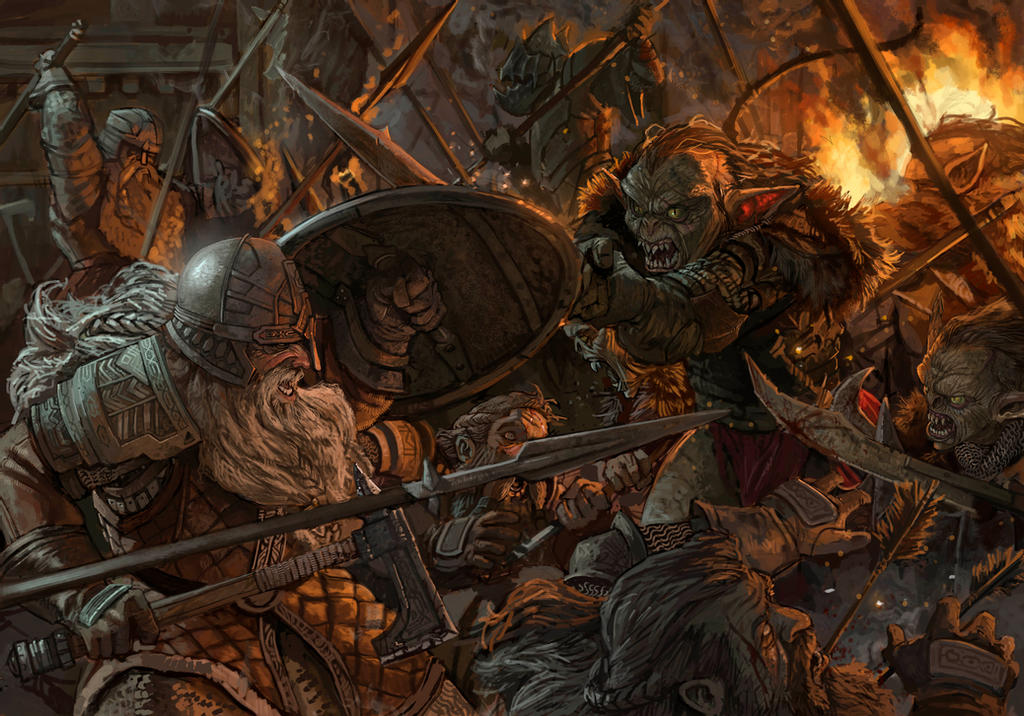
\includegraphics[scale=0.49]{img/the_last_stand_by_ncorva.jpg}
\end{center}
\end{figure*}


\section{Special Combat Rules}

\subsection{Mounted Combat}
A mounted warrior has a +20\% bonus to his attacks and parries against adjacent opponents on foot; a character on foot defending against a mounted attacker suffers a –20\% penalty to his Reaction skill. These modifiers do not apply if the target on foot is as tall (or has a weapon 2 sizes bigger) as the mounted character is. In addition:
\begin{rpg-list}
\item A mounted character uses his mount’s Movement Rate when moving rather than his own.
\item A mounted character charging with a Lance uses his mount’s Damage Modifier rather than his own.
\item A mounted adventurer can use no weapon at a skill level greater than his Riding skill score. 
\end{rpg-list}

\subsubsection{Untrained Mounts}
The rider of a mount unused to combat must make a Riding Skill test at the start of each Combat Round.
On success the horse is treated as a trained mount for the remainder of the Combat Round. 
On failure the horse flees combat (use the Sprint action) at every opportunity for the remainder of the Combat Round. 


\subsection{Two Weapon Use}
A character wielding two weapons or a weapon and a shield may use the off-hand item to either: 
\begin{rpg-list}
\item Parry one additional attack per Combat Round (over and above the normal Reaction allowance)
\item Gain a single bonus Close Combat Attack action. This bonus attack is at -20\% Close Combat Skill. The second attack occurs at half the character’s combat order. Also this may only be a normal Close Combat Attack, not a special attack like All Out Attack, Disarming Attack, Great Attack, etc.
\end{rpg-list}

\begin{rpg-examplebox}
	A warrior armed with sword and shield, can attack with the sword normally at combat order 15 and then follow this up at combat order 8 with a shield bash at -20\% to the shield attack.
\end{rpg-examplebox}



%\subsection{Combat Skills above 100\%}
%A character with over 100\% can split his skill to perform multiple attacks and parries or dodges. The skill percentage can be split anyway the character wants but no attack can be less that 50\%. If you split an attack (close or ranged) you cannot use any special attacks (e.g. Disarm, Great Attack, Aim, etc).

%\begin{rpg-examplebox}
%For example Curgan the Mighty with an Axe skill of 150\% can split it 75\% / 75\% or make three attacks at three opponents in range at 50\% each.
%\end{rpg-examplebox}

%Divide the character’s combat order by the number of attacks to find when attacks occur in the combat order sequence. First attack is at normal combat order and then subsequent attacks are at intervals of combat order divided by the number of attacks.

%\begin{rpg-examplebox}
%Curgan the Mighty with a combat order of 12 splits his attack to make two attacks. Therefore the first attack occurs at combat order 12 and the second at 6.
%\end{rpg-examplebox}

%Parries and Dodges do not need to be declared at the start of combat round but careful track must be kept of how many have already been used.

%\begin{rpg-examplebox}
%Curgan parries one of his attackers and chooses to use 90\% of his skill. This means that he has 60\% left to parry the next attacker in the same round.
%\end{rpg-examplebox}

\begin{table*}
\begin{center}
\caption{Summary of Combat Actions}
\label{tab:summary-of-combat-actions}
\begin{rpg-table}[|l|X|]
        \hline
        \textbf{Action} & \textbf{Description}\\
        \hline
        Charge               & Character moves twice movement, followed by a close combat attack with a +1D6 to damage. Loses Reaction for the round. If charging uphill do not apply the extra damage.\\
        Close Combat Attack  & Character attacks opponent with weapon, tests vs. Close Combat skill. If successful does weapon damage plus damage modifier.\\
        All Out Attack       & Two attacks at -20\%. Gives up Reaction for round.\\
        Great Attack         & One attack at +20\% with maximum damage modifier. Gives up Reaction for round.\\
        Disarming Attack     & Attack at -20\% to disarm opponent. Weapon or shield is thrown 1D6 meters away.\\
        Knockout Attack      & Attack at -20\% to knock out opponent. If the damage is equal to a major wound the target is knocked out. Otherwise minimum weapon damage.\\
	Knock-Back Attack    & Attack with shield (at -20\% if in off-hand). If opponent fails to parry or dodge he is pushed back 2 meters and needs an Athletics roll at -20\% or fall prone.\\
        Set Weapon           & As an action the character sets a spear or polearm in anticipation of a charge. When it occurs the character attacks first with +20\% to weapon skill.\\
        Standard Move        & The character moves their Movement Rate in metres as a free action, once per round.\\
        Change Stance        & May move from prone to standing and vice versa.\\
	Fighting Retreat     & Moves their Movement Rate and defends at +20\% (+40\% if using a Medium or Large Shield).\\
	Sprint               & Moves twice Movement Rate. May not attack and may only Dodge as a reaction.\\
	Ranged Combat Attack & Character attacks opponent with weapon, tests vs. Ranged Combat skill if successful then does weapon damage (plus damage modifier for thrown weapons only).\\
	Ranged Combat Aim    & Character aims for a combat round to gain +20\% to the next ranged attack.\\
	Use Supernatural Power & Character uses a supernatural Power. Cost and effect depends on the Discipline.\\
	Delay                & Character either waits until after another character’s action or tries to interrupt it.\\
	Intimidate/Persuade  & The character uses their Influence skill vs the enemies’ Persistence to either intimidate, or persuade foes who are facing defeat, to flee or surrender.\\
	Ready Weapon         & Character draws or loads weapon making it ready for combat. It takes half his movement to ready a single weapon.\\
	Skill Use            & Character uses a non combat skill.\\
	Unarmed Attack       & The character can either attack using a natural weapon, such as a fist or claw, or grapple.\\
        \hline
\end{rpg-table}
\end{center}
\end{table*}


